\documentclass{beamer}
\usepackage[utf8]{inputenc}
\usepackage{graphicx}

\hypersetup{
    colorlinks,%
    citecolor=blue,%
    filecolor=blue,%
    linkcolor=blue,%
    urlcolor=blue 
    %urlcolor=mygreylink     % can put red here to better visualize the links
}

\author[Sowmya Vajjala]{Instructor: Sowmya Vajjala}

\title[LING 520]{LING 520: Computational Analysis of English}
\subtitle{Semester: FALL '16}

\date{8 November 2016}

\institute{Iowa State University, USA}
%%%%%%%%%%%%%%%%%%%%%%%%%%%

\begin{document}

\begin{frame}\titlepage
\end{frame}

\begin{frame}
\frametitle{Class Outline}
\begin{itemize}
\item Regular expressions on parse trees: references %10 min
\item Semantics: Relevance in NLP %10min
\item Overview of tools and resources in computational semantics %30
\item NLTK Exercises%20 min
\item Reminder 1: Assignment 5 is due on 15th November.
\item Reminder 2: Those who did not submit their 1 page reports - Please talk to me after the class.
\end{itemize}
\end{frame}

\begin{frame}
\frametitle{Regular Expressions on Parse Trees}
\begin{itemize}
\item It is possible to create regular expressions with parse trees (example purpose: patterns of parent-child relationship between nodes) 
\item Tregex is a utility that can work with Stanford parser trees, available for download on Stanford NLP website. \\ \url{http://nlp.stanford.edu/software/tregex.shtml}
\item has a UI that should work on all computers.
\item Tregex also comes with another utility called Tsurgeon, which allows us to edit parse trees in locations matched by a tregex pattern.\pause
\item Very useful if you want to extract some syntactic patterns from parse trees (e.g., "clause" is not a part of constituency trees. But you can extract clause patterns from parse trees using tregex).
\end{itemize}
\end{frame}

\begin{frame}
\frametitle{Semantics: Relevance in NLP}
Semantics is useful in artificial intelligence tasks such as:
\begin{itemize}
\item Making a robot follow written set of instructions 
\item Finding if a student answer is relevant to the question asked
\item Holding a dialogue with user (real dialogue, not like Eliza)
\item Making the computer understand humor, sarcasm, metaphor etc.
\item Tasks like sentiment analysis too may eventually require semantics to understand what the review really means. 
\end{itemize}
\end{frame}

\begin{frame}
\frametitle{How is semantics represented in NLP?}
\begin{itemize}
\item Semantics is studied in using formal systems of logic such as first order logic.
\item Computational semantics follows that same tradition.
\item I am not going into that theoretical details (again, they are taught in separate courses!)
\item If you are primarily a linguist (not an applied linguist) and are trained in logic, you can go through Chapter 10 in NLTK for practical stuff and Chapters 17--21 for a more rigorous treatment of computational semantics. 
\item For the state of the art on research in this topic, view this tutorial: \url{http://yoavartzi.com//pub/afz-tutorial.acl.2013.pdf}
\end{itemize}
\end{frame}

\begin{frame}
\frametitle{How is semantics represented in NLP?}
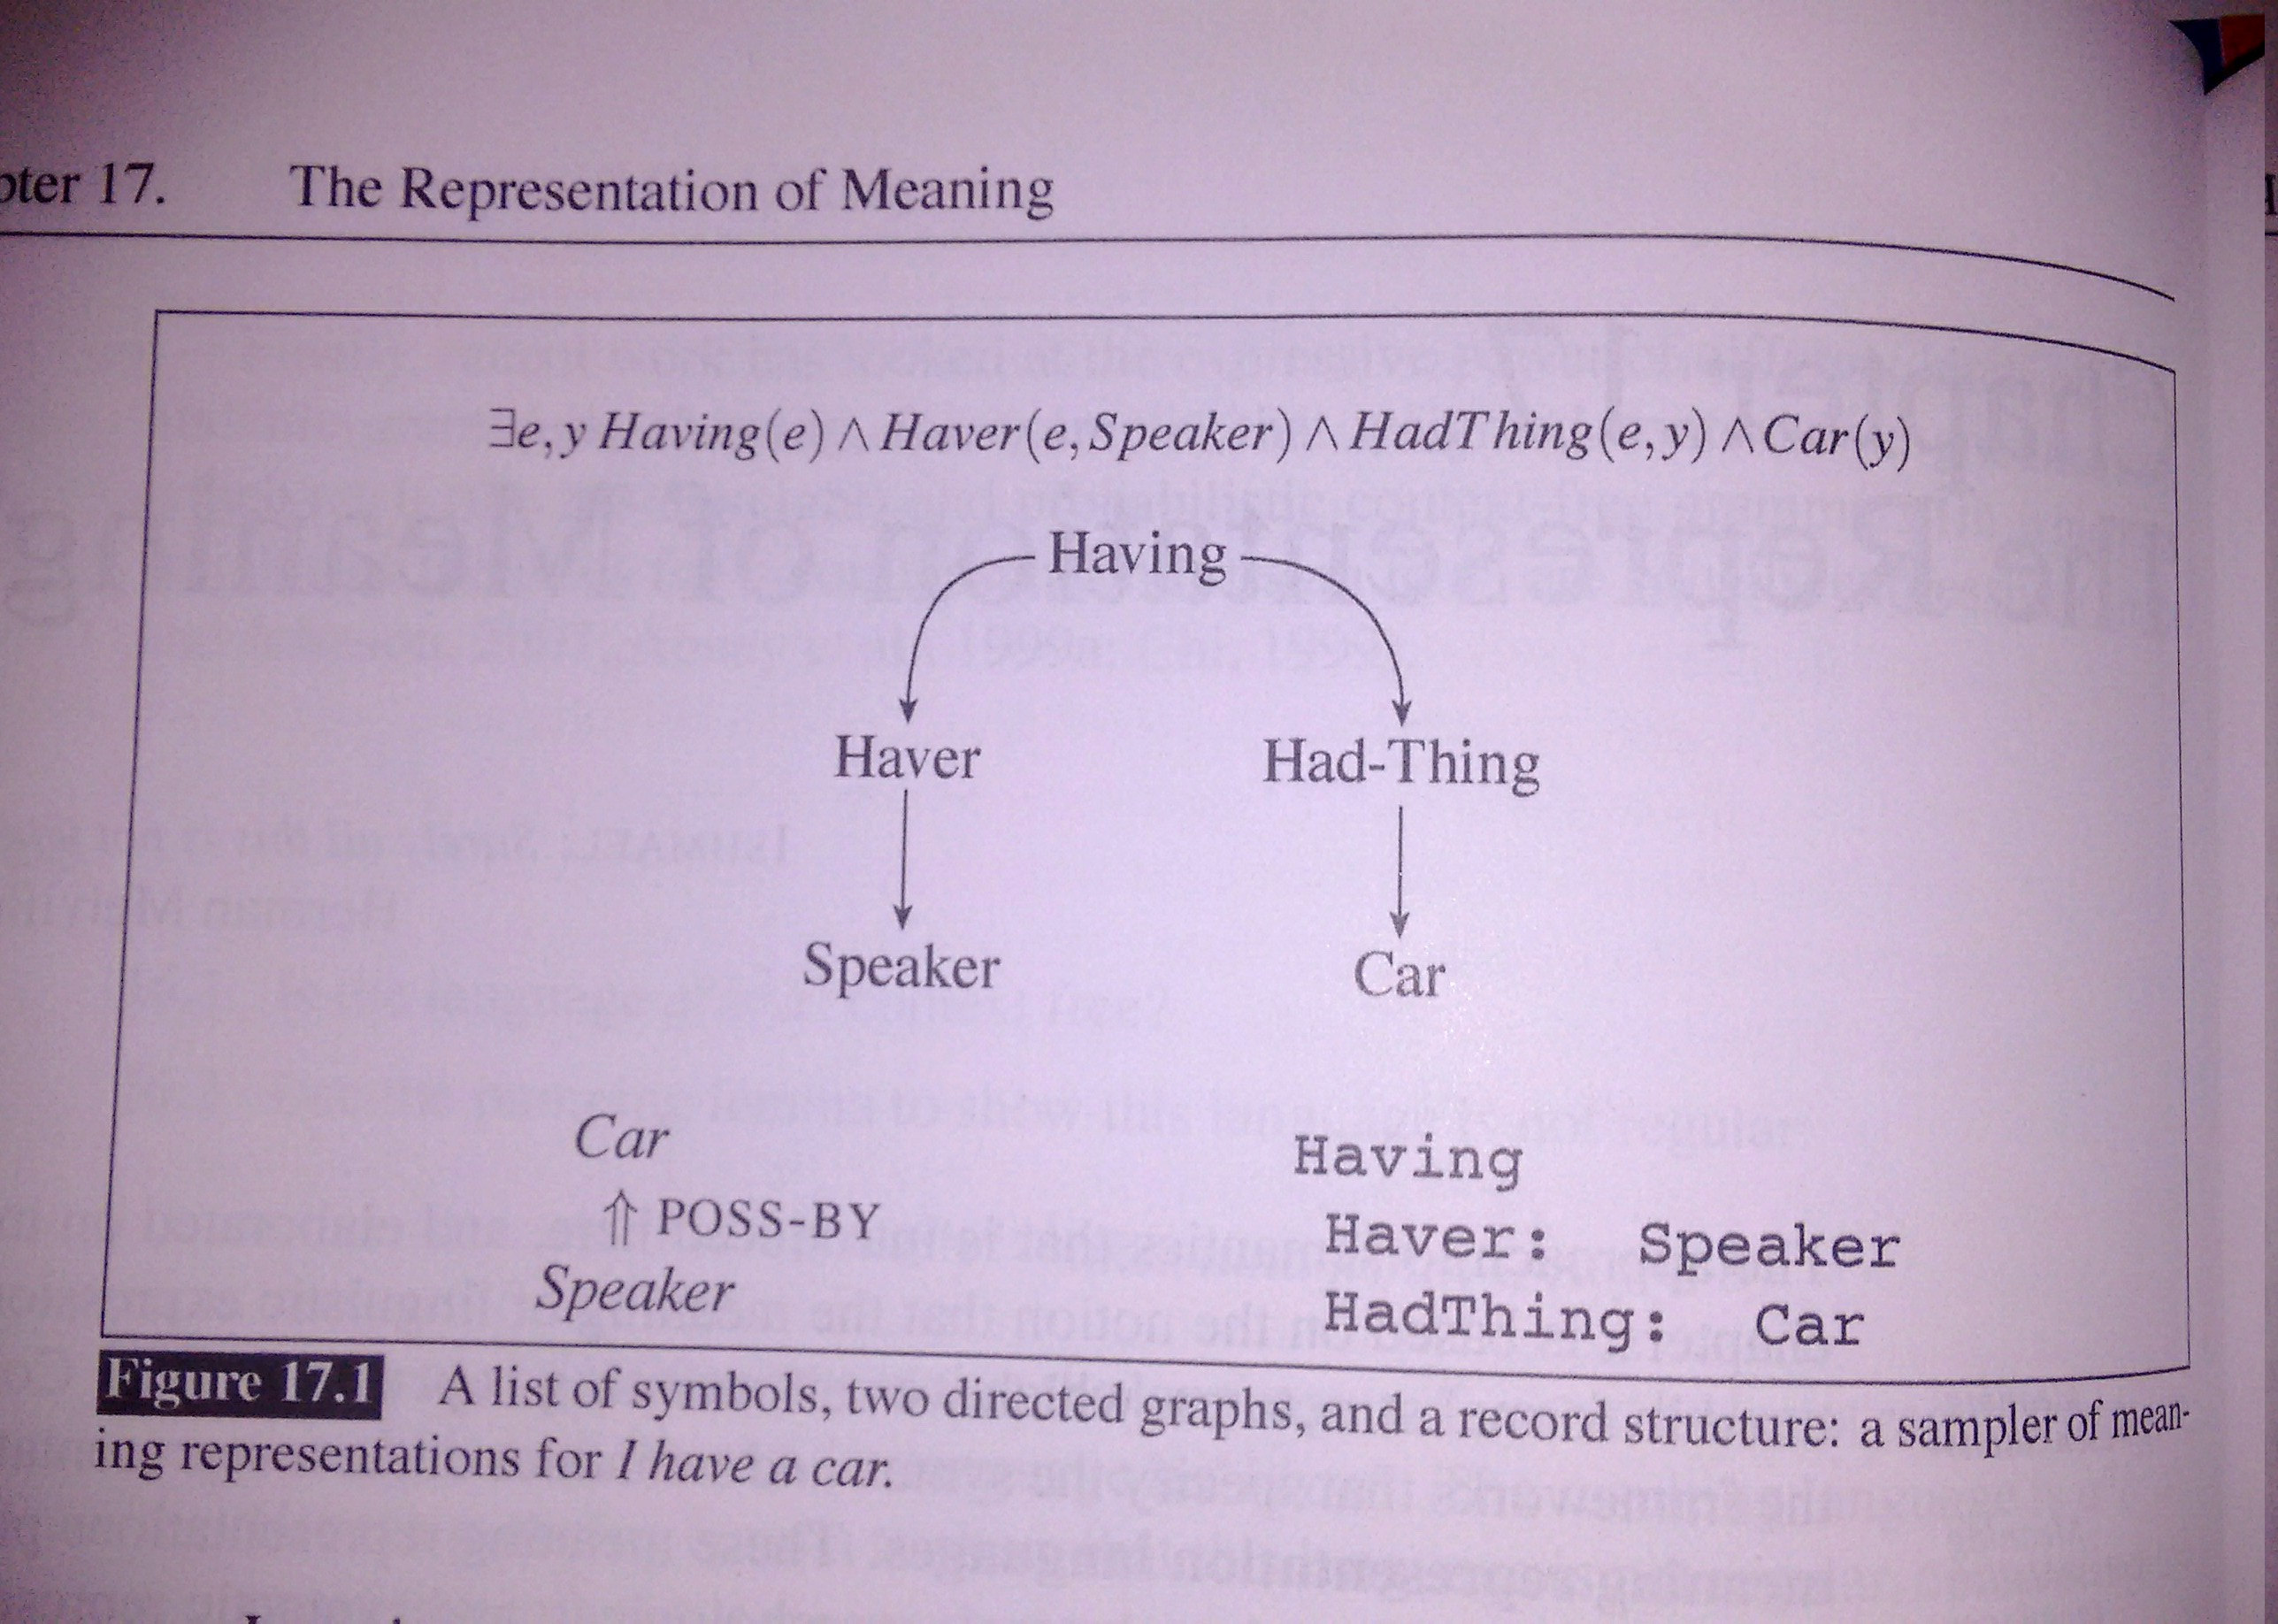
\includegraphics[width=\textwidth]{semantics.jpg}
\end{frame}

\begin{frame}
\frametitle{Semantics in NLP}
\begin{itemize}
\item Lexical semantics - understanding the meaning of words
\item Distributional semantics: "a word is characterized by the company it keeps" (J.R.Firth)
\item Syntax driven semantics - understanding the meaning of sentences
\end{itemize}
\end{frame}

\begin{frame}
\frametitle{Semantics of words: Lexical Semantics in NLP}
\begin{itemize}
\item identifying word sense in context (ambiguous words like bank, for example)
\item identifying different semantic relations between words (eg: synonymy, antonymy, hyponymy, hypernymy, homonymy, polysemy, metonymy, meronymy)
\item identifying different semantic relations between words based on how they are "used" in real word (distributional semantics)
\end{itemize}
\end{frame}

\begin{frame}
\frametitle{Relations between words: Examples}
\begin{itemize}
\item synonymy: good and nice can be considered synonyms
\item antonymy: good and bad are antonyms
\item hyponymy and hypernymy: crow is a hyponym of bird. Bird is a hypernym of crow.
\item homonymy: words having identical form but different meaning
\item polysemy: one word having multiple meanings (differences between homonymy and polysemy.. some examples: \url{https://goo.gl/lbU1D0}) 
\item metonymy: usage of an expression to indicate something closely associated with it. Using Whitehouse to refer to the government administration.
\item meronym: part-of-whole relationships. NLP is a meronym of AI. keys are meronyms of keyboard etc.
\end{itemize}
\end{frame}

\begin{frame}
\frametitle{Resources for Computational Lexical Semantics}
\begin{itemize} \small
\item Wordnet : database of lexical semantic relations between English words. (exists for some other languages as well) \\ \url{https://wordnet.princeton.edu/}
\item VerbNet: a resource for English verbs, based on Levin's verb classes. Links to wordnet. (Beth Levin, the linguist) \\ \url{http://verbs.colorado.edu/~mpalmer/projects/verbnet.html}
\item FrameNet: based on linguistic theories on "frame semantics", which uses something called "frame" to describe a event. For example, the frame about "food" may have elements: cook, thing being cooked, source of heat etc. \\ (\url{https://framenet.icsi.berkeley.edu/fndrupal/about})
\item Typically, such resources are used to do word sense disambiguation, and for deriving information about similarity between words (useful in various NLP tasks including essay grading) 
\end{itemize}
.. resources are starting to emerge for other languages as well. But most work is in English. 
\end{frame}

\begin{frame}
\frametitle{Semantics of words: Distributional Semantics in NLP}
\begin{itemize}
\item Idea: derive information about semantic similarity of words by studying their usage in context in large corpora
\item Example: if I have several sentences about pets, after applying some distributional semantics method, a computer should understand dogs, cats, horses etc are all pets people have. 
\item Use: particularly useful for covering words not covered by resources like wordnet. Also useful for doing NLP with languages that do not have such fancy resources.
\item How?: Collecting contexts of appearance of words (n words before and/or after a given word), calculating what other words have similar contexts. 
\item typical methods: latent semantic analysis, word embeddings etc (discussed in detail in 515)
\item Python has libraries that can do distributional semantics.
\end{itemize}
\end{frame}

\begin{frame}
\frametitle{Syntax driven semantic analysis}
\begin{itemize}
\item idea: meaning of a sentence is not purely based on meaning of the words in it, but on the ordering and grouping of words and relations between them.
\item that is, meaning needs syntactic structure.
\item Process: augment a CFG with semantic rules that specify how to get the meaning representation based on syntax. 
\end{itemize}
\end{frame}

\begin{frame}
\frametitle{Semantics enhanced parsing rules}
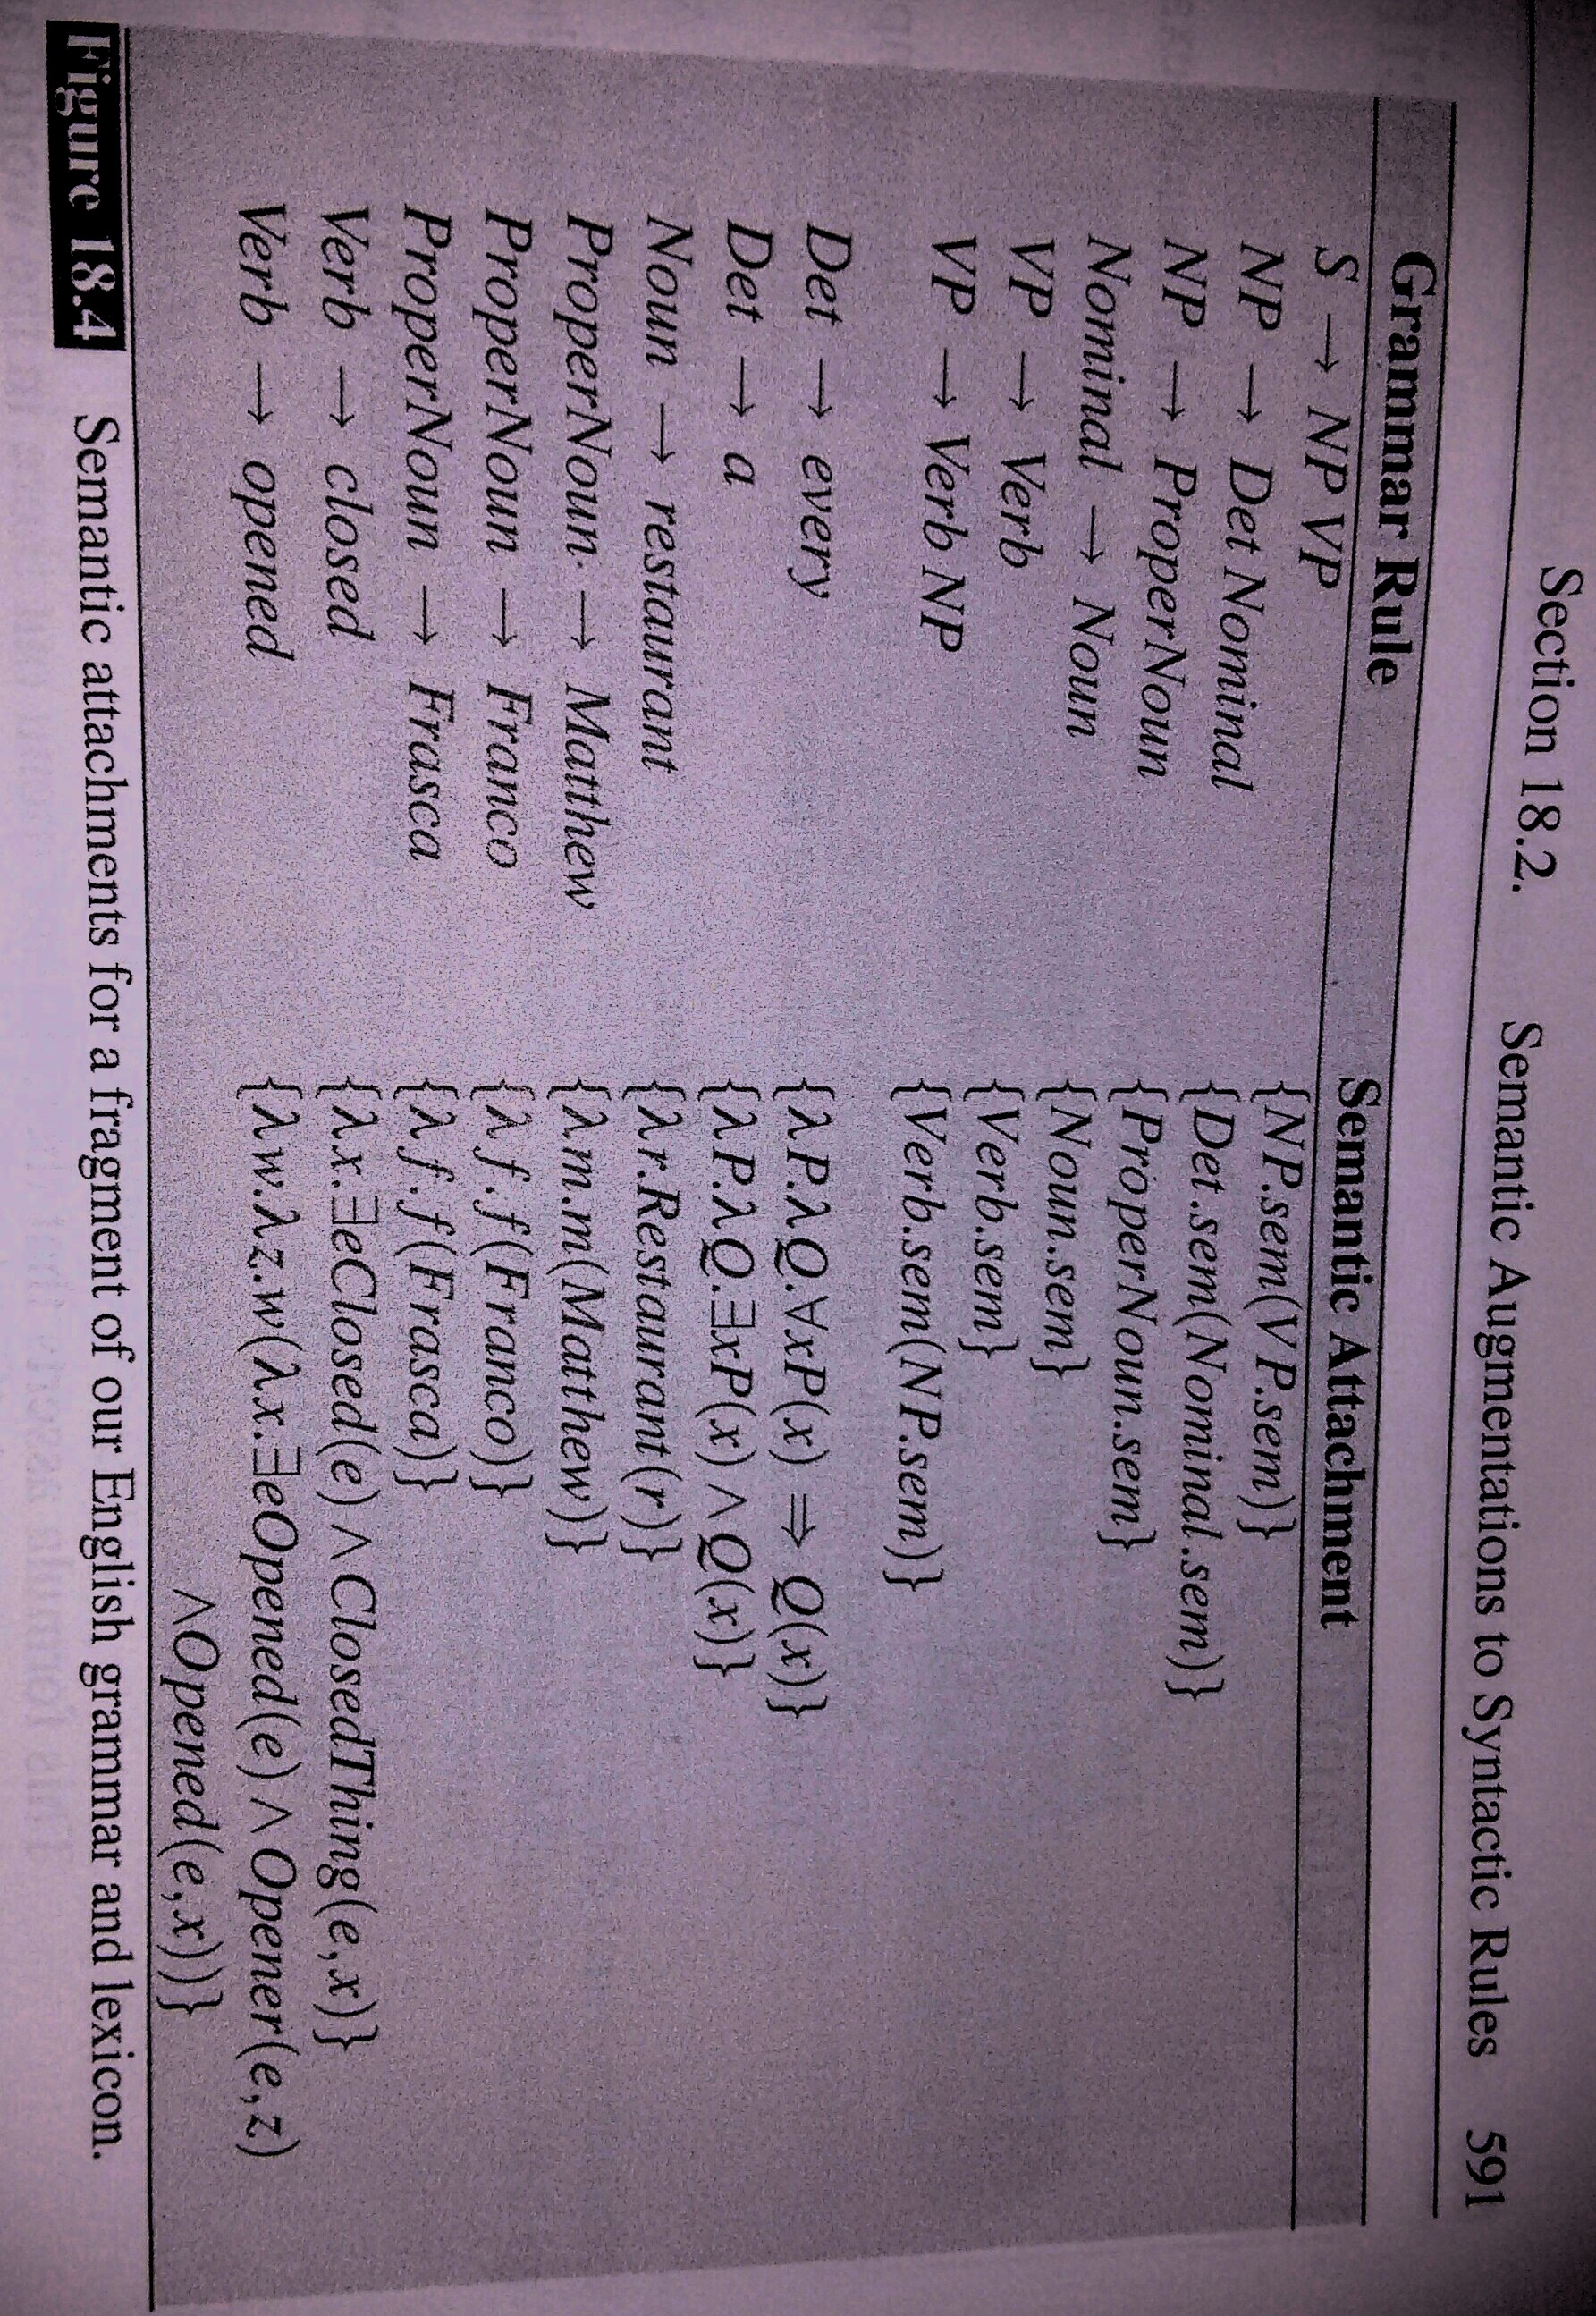
\includegraphics[angle=90,width=\textwidth]{semanticrules.jpg}
\end{frame}

\begin{frame}
\frametitle{Meaning of sentences}
Semantically parsing sentences. 
\begin{itemize}
\item \url{https://goo.gl/9nltNU}
\item \url{http://cogcomp.cs.illinois.edu/page/demo_view/srl}
\item \url{http://barbar.cs.lth.se:8081/parse}
\item Resource: PropBank - resource of sentences annotated with semantic roles (English and Chinese)
\\ \url{https://www.researchgate.net/figure/283893596_fig3_Fig-19-Sample-PropBank-entry}
\end{itemize}
\end{frame}


\begin{frame}
\frametitle{Exercises}
Exercises I am going to give today and from now on will be more open-ended and undirected, for two reasons: 
\begin{enumerate}
\item We are into Week 12, and I want you to "think" more rather than doing what I tell you to do. 
\item I don't know what specific problems you are interested in and where do these issues like semantics come into picture in that.
\end{enumerate}
\end{frame}

\begin{frame}
\frametitle{Exercise 1: NLTK exercises}
\begin{itemize}
\item Chapter 3, Section 5 in NLTK demonstrates what we can do with WordNet in NLTK.
\item Practice the examples there, and come up with problems in your topic of interest where you may find such a resource useful.
\item In about 20 minutes, I want some of you to comment on what scenarios you thought about for using wordnet.
\end{itemize}
\end{frame}

\begin{frame}
\frametitle{Exercise 2: using Tregex}
\begin{itemize}
\item Download tregex, check if you can use the interface and run the program without problems.
\item Following the power point slides on Stanford Tregex page, learn to use the tool to extract patterns from trees.
\item If you are interested, read this 2006 short article that describes these two tools for the first time: \url{http://nlp.stanford.edu/pubs/levy_andrew_lrec2006.pdf}
\item Figure out if you can use it in Python code somehow.
\end{itemize}
\end{frame}
\end{document}

%Thursday: Discourse
%\item Overview of NLP applications: Machine Translation, Topic Modeling, Question Answering etc. 
%One way: take task yb task: wsd, ner, srl, discourse analysis etc - get examples of code-software to talk about.
%MT: Talk about Moses and Apertium
%LG: NLG

\begin{frame}
\frametitle{Programming exercise - 1}
\begin{itemize}
\item Take any .txt version file from gutenberg.org, written by your favorite author (in English!)
\item Read that file into your python code, and do the following using NLTK:
\begin{enumerate}
\item Split the file into sentences.
\item Print the following: number of sentences in the file, average sentence length (in number of words), average word length (in number of characters), number of unique words, number of unique stems.
\item Note 1: Once sentence splitting is done, you can ignore punctuation markers for the rest of the calculation.
\item Note 2: You can use any stemmer you want.
\end{enumerate}
\end{itemize}
\end{frame}

\begin{frame}
\frametitle{Programming exercise - 1}
\begin{itemize}
\item For the same file from last slide, do the following:
\item Read that file into your python code, and do the following using NLTK:
\begin{enumerate}
\item Split the file into sentences.
\item For each sentence, print its POS tagged version as a string of tags. E.g., if you have "It is a sentence" as your sentence, and your NLTK tagger outputs the tags for this sentence as a list (or tuple or whatever), you should print the tag as a string. E.g., PRP VBZ DT NN (not as [PRP, VBZ, DT, NN] or as [(It, PRP), (is, VBZ) .. ... ])
\end{enumerate}
\end{itemize}
\end{frame}
